\chapter{几何Satake等价II：等变反常层范畴的张量结构}\label{L22}\lecturedate{2020/05/06}\sourcepage{182}
设$k=\C$；关于$k$为一般交换环的情形，参见\bref{L22MV}{MV}。设$G$为分裂约化群，分别记$\mathcal K=k((t))$、$\mathcal O=k[[t]]$。仿射Grassmannian的点集可识别为$G(\mathcal K)/G(\mathcal O)$。

如\lref{L21}所定义，$P_{G(\mathcal O)}(\operatorname{Gr},k)$为仿射Grassmannian上$k$系数的$G(\mathcal O)$等变反常层范畴。回忆，$\operatorname{Gr}$通常为无限维，但它具有由有限维$G(\mathcal O)$轨道组成的分层$\mathcal S$：
\begin{equation}\tag{0.1}\label{L22eq01}\operatorname{Gr}=\bigsqcup_{\lambda\in(X^\vee)^+}\operatorname{Gr}_\lambda,\qquad\operatorname{Gr}_\lambda=G(\mathcal O)\cdot L_\lambda.\end{equation}
这里$\dim\operatorname{Gr}_\lambda=2\langle\kappa,\lambda\rangle$，$\kappa$为$G$的正根之和的一半。令$P_{\mathcal S}(\operatorname{Gr},k)$为相对于这些轨道可构造、具有有限维支撑的反常层范畴。由\eref{命题}{L21S3O1}，有以下结果。
\originalnumber{1}
\begin{proposition}\label{L22S0O1}范畴$P_{G(\mathcal O)}(\operatorname{Gr},k)$与$P_{\mathcal S}(\operatorname{Gr},k)$自然等价。\end{proposition}
\eqref{L22eq01}是约化群Cartan分解的对应物。还有Iwasawa分解的对应物：
\begin{equation}\tag{0.2}\label{L22eq02}\operatorname{Gr}=\bigsqcup_{\gamma\in X^\vee}S_\gamma,\end{equation}
其中$S_\gamma=N(\mathcal K)\cdot L_\gamma$，$N$为固定Borel子群$B$的幂幺根基。
\sourcepage{183}
以$D_{G(\mathcal O)}(\operatorname{Gr},k)$表示$\operatorname{Gr}$上具有有限维支撑的$G(\mathcal O)$等变可构造$k$层的有界导出范畴。由\lref{L21}末列出的性质，得到以下反常性判据。
\originalnumber{2}
\begin{lemma}\label{L22S0O2}对$\mathcal A\in D_{G(\mathcal O)}(\operatorname{Gr},k)$，下列两条等价：
\begin{enumerate}[label=(\roman*)]
\item $\mathcal A$为反常层。
\item 对所有$\gamma\in X^\vee$，$H_c^*(S_\gamma,\mathcal A)$只可能在次数$2\langle\kappa,\gamma\rangle$非零。
\end{enumerate}
\end{lemma}
\begin{proof}
由\lref{L21}末的性质，对反常层$\mathcal P$，$H_c^m(S_\gamma,\mathcal P)\ne0$蕴含$m=2\langle\kappa,\gamma\rangle$。对任意$\mathcal A$，以${}^pH^j(\mathcal A)$表示其第$j$个反常上同调。$\mathcal A$反常当且仅当所有$j\ne0$时${}^pH^j(\mathcal A)=0$。

由反常上同调的谱序列及上述消失性，得到自然同构
\[H_c^{2\langle\kappa,\gamma\rangle}(S_\gamma,{}^pH^j(\mathcal A))\cong H_c^{2\langle\kappa,\gamma\rangle+j}(S_\gamma,\mathcal A).\]
因此
\begin{align*}
\text{(i)}&\Longleftrightarrow{}^pH^j(\mathcal A)=0\quad(j\ne0)\\
&\Longleftrightarrow H_c^{2\langle\kappa,\gamma\rangle}(S_\gamma,{}^pH^j(\mathcal A))=0\quad(j\ne0,\ \gamma\in X^\vee)\\
&\Longleftrightarrow H_c^{2\langle\kappa,\gamma\rangle+j}(S_\gamma,\mathcal A)=0\quad(j\ne0,\ \gamma\in X^\vee)\\
&\Longleftrightarrow\text{(ii)}.
\end{align*}
\end{proof}
\section{卷积积}\label{L22S1}\idx{反常层的卷积}
在Satake同构的几何表述中，$P_{G(\mathcal O)}(\operatorname{Gr},k)$替代Hecke代数，因此需要在对象上定义对应于交换代数乘法的运算，即为反常层$\mathcal A_1,\mathcal A_2$定义\textbf{卷积积}\znote{卷积积是 Hecke 代数乘法的几何化。在 Hecke 代数中，双陪集上的紧支撑函数按卷积 $(f_1*f_2)(g)=\int f_1(h)f_2(h^{-1}g)\,dh$ 相乘；几何版把函数换成反常层，用图 $\operatorname{Gr}\times\operatorname{Gr}\leftarrow G(\mathcal K)\times\operatorname{Gr}\rightarrow G(\mathcal K)\times^{G(\mathcal O)}\operatorname{Gr}\rightarrow\operatorname{Gr}$ 上的拉回与真推前代替积分。易错点：两个步骤都只在层上操作，卷积不能逐点定义；需要先验证所得层反常，这正是命题 1.3 的内容。[来源：nLab \textquotedbl geometric Satake equivalence\textquotedbl，\url{https://ncatlab.org/nlab/show/geometric+Satake+equivalence}（Last revised 2024-07-22；2026-11-14 访问）。]}$\mathcal A_1*\mathcal A_2$。
\sourcepage{184}
考虑下列映射图：
\begin{figure}[H]\centering\begin{equation}\tag{1.1}\label{L22eq11}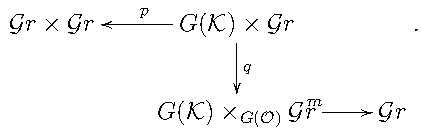
\includegraphics[width=0.3404\paperwidth]{images/L22-p184-convolution.pdf}\end{equation}\end{figure}
这里$G(\mathcal K)\times^{G(\mathcal O)}\operatorname{Gr}$为$G(\mathcal K)\times\operatorname{Gr}$关于$G(\mathcal O)$作用的商，该作用在第一因子为右乘逆元，在第二因子为左乘。\eqref{L22eq11}中$p=p_G\times\operatorname{id}_{\operatorname{Gr}}$，其中$p_G:G(\mathcal K)\to\operatorname{Gr}$为商映射；$q$为上述对角作用的商映射；$m$为乘法映射。定义
\begin{equation}\tag{1.2}\label{L22eq12}\mathcal A_1*\mathcal A_2:=Rm_*\widetilde{\mathcal A},\qquad q^*\widetilde{\mathcal A}=p^*(\mathcal A_1\boxtimes\mathcal A_2).\end{equation}
也可以说，$\widetilde{\mathcal A}$是$p^*(\mathcal A_1\boxtimes\mathcal A_2)$下降到$G(\mathcal K)\times^{G(\mathcal O)}\operatorname{Gr}$后得到的层。注意，$\mathcal A_1,\mathcal A_2$都$G(\mathcal O)$等变，因此$p^*(\mathcal A_1\boxtimes\mathcal A_2)$为$G(\mathcal O)\times G(\mathcal O)$等变层\znote{等变层是带 $G$ 作用的空间 $X$ 上的层 $\mathcal F$，附带同构 $\alpha:a^*\mathcal F\cong\operatorname{pr}^*\mathcal F$（$a:G\times X\to X$ 为作用映射），并要求 $\alpha$ 在结合律意义下满足余圈条件；等价的说法是 $X/G$（或商叠）上的层。易错点：等变结构是附加数据而非层的性质，同一个底层的层可以带不同的等变结构；只有当作用自由时，下降才唯一地把等变层等同于商上的层。[来源：nLab \textquotedbl equivariant sheaf\textquotedbl，\url{https://ncatlab.org/nlab/show/equivariant+sheaf}（Last revised 2024-12-24；2026-11-14 访问）。]}：第一群在$G(\mathcal K)$因子上左乘，第二群按$q$所商掉的对角作用（$G(\mathcal K)$上右乘逆元、$\operatorname{Gr}$上左乘）作用。由于第二群的作用自由，这个等变层唯一地下降到商空间。

赋予$G(\mathcal K)\times^{G(\mathcal O)}\operatorname{Gr}$分层$\mathcal T$，其层为
\begin{equation}\tag{1.3}\label{L22eq13}\widetilde{\operatorname{Gr}}_{\lambda,\gamma}:=p_G^{-1}(\operatorname{Gr}_\lambda)\times^{G(\mathcal O)}\operatorname{Gr}_\gamma.\end{equation}
注意，$\dim\widetilde{\operatorname{Gr}}_{\lambda,\gamma}=2\langle\kappa,\lambda+\gamma\rangle$。
\originalnumber{1}
\begin{lemma}\label{L22S1O1}若$\mathcal A_1,\mathcal A_2$反常，则$\widetilde{\mathcal A}$相对于分层$\mathcal T$反常。\end{lemma}
\begin{proof}
按定义，只需在每个$\widetilde{\operatorname{Gr}}_{\lambda,\gamma}$上检查支撑与余支撑条件。记其包含映射为$i_{\lambda,\gamma}$，$d_{\lambda,\gamma}=2\langle\kappa,\lambda+\gamma\rangle$，则条件为
\[\begin{cases}\mathcal H^j(i_{\lambda,\gamma}^*\widetilde{\mathcal A})=0,&j>-d_{\lambda,\gamma},\\\mathcal H^j(i_{\lambda,\gamma}^!\widetilde{\mathcal A})=0,&j<-d_{\lambda,\gamma}.\end{cases}\]
在$p$与$q$的局部平凡化中，这等价于$\mathcal A_1\boxtimes\mathcal A_2$在$\operatorname{Gr}_\lambda\times\operatorname{Gr}_\gamma$上的同样两个条件：
\[\begin{cases}\mathcal H^j(i_{\operatorname{Gr}_\lambda\times\operatorname{Gr}_\gamma}^*(\mathcal A_1\boxtimes\mathcal A_2))=0,&j>-d_{\lambda,\gamma},\\\mathcal H^j(i_{\operatorname{Gr}_\lambda\times\operatorname{Gr}_\gamma}^!(\mathcal A_1\boxtimes\mathcal A_2))=0,&j<-d_{\lambda,\gamma}.\end{cases}\]
% [Tutor Note: 原书 p184 证明中第二个条件作 $\mathcal H^j_c(\widetilde{\mathcal A}|_{\widetilde{\operatorname{Gr}}_{\lambda,\gamma}})=0,\ \forall j<2\langle\kappa,\lambda+\gamma\rangle$；按中围反常性（即第 21 讲末所列两条消失性质）应为 $\mathcal H^j(i_{\lambda,\gamma}^!\widetilde{\mathcal A})=0,\ \forall j<-2\langle\kappa,\lambda+\gamma\rangle$，译文按标准写法处理。]
\sourcepage{185}
所以只需证明导出外张量积$\mathcal A_1\boxtimes^L\mathcal A_2$相对于$\operatorname{Gr}\times\operatorname{Gr}$上的分层$\mathcal S\times\mathcal S$反常。由\eref{命题}{L22S0O1}与\eref{引理}{L22S0O2}的乘积版本，只需证明
\[H_c^n(S_\gamma\times S_\nu,\mathcal A_1\boxtimes\mathcal A_2)=0,\qquad n\ne2\langle\kappa,\gamma+\nu\rangle.\]
这由Künneth公式
\[H_c^n(S_\gamma\times S_\nu,\mathcal A_1\boxtimes\mathcal A_2)\cong\bigoplus_{n_1+n_2=n}H_c^{n_1}(S_\gamma,\mathcal A_1)\otimes H_c^{n_2}(S_\nu,\mathcal A_2),\]
以及$H_c^n(S_\eta,\mathcal A_i)=0$，$i=1,2$、$n\ne2\langle\kappa,\eta\rangle$，立即得到。
\end{proof}
\originalnumber{2}
\begin{note}[L22S1O2]
一般而言，若$k$不是域，则\eqref{L22eq12}中$\widetilde{\mathcal A}$的定义应改为
\[q^*\widetilde{\mathcal A}=p^*\bigl({}^pH^0(\mathcal A_1\boxtimes^L\mathcal A_2)\bigr).\]
\end{note}
\originalnumber{3}
\begin{proposition}\label{L22S1O3}若$\mathcal A_1,\mathcal A_2$反常，则其卷积积$\mathcal A_1*\mathcal A_2$反常。\end{proposition}
为了证明这一命题，先介绍\textbf{分层半小映射}\znote{半小映射的直觉是：目标层 $T_2$ 上纤维的维数受源层 $\overline{T_1}$ 的余维控制，即 $\dim(f^{-1}(x)\cap\overline{T_1})\le\frac12(\dim\overline{T_1}-\dim T_2)$。它等价于 $\dim(X\times_YX)\le\dim X$，也等价于 $\operatorname{codim}_Y\{y:\dim f^{-1}(y)\ge r\}\ge2r$（命题 1.5）。易错点：条件必须用闭包 $\overline{T_1}$（开层本身不闭），且要求 $f|_{\overline{T_1}}$ 真，否则维数估计失去意义。半小映射的分解定理是本讲把卷积层拆成 IC 层直和的关键。[来源：de Cataldo--Migliorini, \textit{The decomposition theorem, perverse sheaves and the topology of algebraic maps}, \S4.2（本讲参考文献）。]}。设$(Y_1,\mathcal T_1)$、$(Y_2,\mathcal T_2)$为分层复空间。
\begin{definition*}
若每个$T_1\in\mathcal T_1$的像$f(T_1)$都是$\mathcal T_2$中若干层的并，并且对每个$T_2\in\mathcal T_2$，$f^{-1}(T_2)\to T_2$为拓扑局部平凡纤维化，则称$f:Y_1\to Y_2$为相对于这两个分层的\textbf{分层映射}。若还满足以下条件，则称其为\textbf{分层半小映射}：
\begin{enumerate}[label=\arabic*.]
\item 对每个$T_1\in\mathcal T_1$，$f|_{\overline{T_1}}$为真映射；
\item 对任意$T_1\in\mathcal T_1$与满足$T_2\subseteq f(\overline{T_1})$的任意$T_2\in\mathcal T_2$，以及对$T_2$中任意一点$x$，有
\[\dim\bigl(f^{-1}(x)\cap\overline{T_1}\bigr)\le\frac12\bigl(\dim\overline{T_1}-\dim T_2\bigr).\]
\end{enumerate}
由局部平凡性，在$T_2$内任取一点的结果相同。
\end{definition*}\idx{半小映射}
% [Tutor Note: 原书 p185 半小映射条件 2 的不等式右端作 $\frac12(\dim f(\overline{T_1})-\dim T_2)$，其中的像维数应为源层维数 $\frac12(\dim\overline{T_1}-\dim T_2)$，否则爆破等标准例子不满足该条件；译文按后者处理。]
\sourcepage{186}
\begin{definition*}
若存在非空的开稠密分层子集$W\subseteq Y_1$，满足以下条件，则称$f$为\textbf{分层小映射}：
\begin{enumerate}[label=\arabic*.]
\item 对每个$T_1\in\mathcal T_1$，$f|_{\overline{T_1}}$为真映射；
\item $f|_W:W\to f(W)$有限，并且$W=f^{-1}(f(W))$，其中$f(W)$为目标中的开稠密分层部分；
\item 对任意$T_1\in\mathcal T_1$与满足$T_2\subseteq f(\overline{T_1})\setminus f(W)$的任意$T_2\in\mathcal T_2$，以及对$T_2$中任意一点$x$，有
\[\dim\bigl(f^{-1}(x)\cap\overline{T_1}\bigr)<\frac12\bigl(\dim\overline{T_1}-\dim T_2\bigr).\]
\end{enumerate}
\end{definition*}\idx{小映射}
% [Tutor Note: 原书 p186 小映射定义先引入开稠密分层子集 $U\subset Y_1$，条件 2、3 中却改记为 $W$（$U,W$ 混用）；译文统一记为 $W$。]
\originalnumber{4}
\begin{lemma}\label{L22S1O4}
若$f$为分层半小映射，则对任意$\mathcal A\in P_{\mathcal T_1}(Y_1,k)$，$Rf_*\mathcal A\in P_{\mathcal T_2}(Y_2,k)$。若$f$为分层小映射，$W$如上，$\mathcal A$为$W$上的反常层，则
\[Rf_*j_{!*}\mathcal A\cong\widetilde j_{!*}(f|_W)_*\mathcal A,\]
其中$j:W\hookrightarrow Y_1$、$\widetilde j:f(W)\hookrightarrow Y_2$为开包含映射，$j_{!*}$、$\widetilde j_{!*}$为反常中间延拓，见\sref{L13S3}。
\end{lemma}
该引理可由直接的维数估计得到；在下述分解定理适用的情形，也可结合\eref{定理}{L22S1O8}与\eref{定理}{L13S3O4}理解这一结论。

下面暂时讨论一般的半小映射。更详细的内容可见\bref{L22dCM}{dCM}第4.2节。
\originalnumber{5}
\begin{proposition}\label{L22S1O5}
设$X$为连通非奇异$n$维簇，$f:X\to Y$为真满态射。设$Y=\bigsqcup_k S_k$为适合$f$的分层，即$f^{-1}(S_k)\to S_k$拓扑局部平凡。取$y_k\in S_k$，令$d_k=\dim f^{-1}(y_k)=\dim f^{-1}(S_k)-\dim S_k$。以下条件等价：
\begin{enumerate}[label=\arabic*.]
\item $Rf_*\Q_X[n]$为$Y$上的反常层；
\item $\dim(X\times_YX)\le n$；
\item 对每个层$S_k$，$\dim S_k+2d_k\le\dim X$；
\item 对任意$r\ge1$，$\operatorname{codim}_Y\{y\in Y\mid\dim f^{-1}(y)\ge r\}\ge2r$。
\end{enumerate}
\end{proposition}
\sourcepage{187}
满足\eref{命题}{L22S1O5}中任一等价条件的真满态射称为\textbf{半小映射}。若$\dim S_k+2d_k=\dim X$，则称层$S_k$为\textbf{相关层}。还有以下小映射的定义。
\originalnumber{6}
\begin{definition}\label{L22S1O6}
簇之间的真满态射$f:X\to Y$称为\textbf{小映射}，若其满足以下任一等价条件：
\begin{enumerate}[label=\arabic*.]
\item 存在开稠密子集$U\subseteq Y$，使$f^{-1}(U)\to U$有限，并且
\[\dim\bigl((X\times_YX)\setminus(f^{-1}(U)\times_Uf^{-1}(U))\bigr)<\dim X;\]
\item 对任意$r\ge1$，$\operatorname{codim}_Y\{y\in Y\mid\dim f^{-1}(y)\ge r\}>2r$；
\item 每个层都满足$\dim S_k+2d_k\le\dim X$，而且每个在$Y$中不稠密的层都不是相关层，即满足严格不等式$\dim S_k+2d_k<\dim X$。
\end{enumerate}
特别地，小映射都是半小映射。
\end{definition}
% [Tutor Note: 原书 p187 定义 1.6 条件 1 作 $\dim(X\times_YX-\Delta_X)<\dim X$；它与条件 2、3 并不等价（取有限二重覆叠即得反例：小映射成立而条件 1 不成立），译文按 de Cataldo--Migliorini 的标准表述处理。]
\originalnumber{7}
\begin{note}[L22S1O7]半小映射在一般点上有限，反之不成立。例如，$\C^3$中一点的爆破。\end{note}
回忆，$IC_X^\bullet\mathbb V[n]$为$X$上的反常层，称为局部系统$\mathbb V$的反常延拓，见\sref{L13S3}。这种形式的反常层也称为\textbf{IC层}。由\eref{定理}{L13S3O4}，它们是构成$\operatorname{Perv}(X)$中对象的基本组成部分。
\originalnumber{8}
\begin{theorem}\label{L22S1O8}
\begin{enumerate}[label=(\arabic*)]
\item 若$f:X\to Y$为小映射，且在一般点的次数为$1$，则
\[Rf_!IC_X^\bullet\Q[n]\cong IC_Y^\bullet\Q[n],\qquad n=\dim X=\dim Y.\]
特别地，$\operatorname{IH}^j(Y)\cong\operatorname{IH}^j(X)$，其中$\operatorname{IH}^j(Y)$为第$j$个交上同调，即未平移交复形的超上同调$\mathbb H^j(Y,IC_Y^\bullet\Q)$。
\item 若$f:X\to Y$为小映射，$\mathbb V$为源的光滑稠密部分上的局部系统，则
\[Rf_*(IC_X^\bullet\mathbb V[n])\cong IC_Y^\bullet((f|_U)_*\mathbb V)[n],\]
其中$U$取为$f$有限且局部系统定义的适当稠密部分。
\item \textbf{半小映射的分解定理。}对兼容分层的半小映射，$Rf_*(IC_X^\bullet\mathbb V[n])$为反常层。特别地，当$X$光滑且系数为$\Q$时，
\[Rf_*\Q_X[n]\cong\bigoplus_{S_k\text{ 相关}}IC_{\overline{S_k}}^\bullet\mathbb V_k[n-2d_k],\]
其中$\mathbb V_k$为相关层上纤维最高维上同调给出的局部系统。
\end{enumerate}
\end{theorem}\idx{分解定理}\idx{交上同调}
现在回到乘法映射$m:G(\mathcal K)\times^{G(\mathcal O)}\operatorname{Gr}\to\operatorname{Gr}$。源的分层为$\mathcal T=\{\widetilde{\operatorname{Gr}}_{\lambda,\gamma}\}$，其层由\eqref{L22eq13}定义；目标的分层为$\mathcal S=\{\operatorname{Gr}_\lambda\}$。
\sourcepage{188}
\originalnumber{9}
\begin{lemma}\label{L22S1O9}乘法映射$m$相对于上述分层为分层半小映射。\end{lemma}
\begin{proof}
首先，$m(\widetilde{\operatorname{Gr}}_{\lambda,\gamma})$为若干$G(\mathcal O)$轨道的并，包含$\bigcup_{w\in W}\operatorname{Gr}_{\lambda+w(\gamma)}$，并以$\operatorname{Gr}_{\lambda+\gamma}$为稠密轨道。回忆
\[\overline{\operatorname{Gr}_\lambda}=\bigsqcup_{\substack{\nu\in(X^\vee)^+\\\nu\le\lambda}}\operatorname{Gr}_\nu.\]
因此
\[\overline{\widetilde{\operatorname{Gr}}_{\lambda,\gamma}}=\bigsqcup_{\substack{\nu,\theta\in(X^\vee)^+\\\nu\le\lambda,\ \theta\le\gamma}}\widetilde{\operatorname{Gr}}_{\nu,\theta}.\]
更精确地，$\operatorname{Gr}_\xi\subseteq m\bigl(\overline{\widetilde{\operatorname{Gr}}_{\lambda,\gamma}}\bigr)$当且仅当存在$w_1,w_2\in W$及$0\le\lambda'\le\lambda$、$0\le\gamma'\le\gamma$使$w_1(\xi)=\lambda'+w_2(\gamma')$。乘法在这一闭有界卷积空间上的像为$\overline{\operatorname{Gr}_{\lambda+\gamma}}$。它是射影的有界空间，因此$m|_{\overline{\widetilde{\operatorname{Gr}}_{\lambda,\gamma}}}$为真映射。

映射
\[m^{-1}(\operatorname{Gr}_\xi)\xrightarrow{(p_G,m)}\operatorname{Gr}\times\operatorname{Gr}_\xi,\qquad[g,hG(\mathcal O)]\longmapsto(gG(\mathcal O),ghG(\mathcal O))\]
为同构，其逆映射把$(gG(\mathcal O),zG(\mathcal O))$送到$[g,g^{-1}zG(\mathcal O)]$。从而$m$在各目标轨道上为局部平凡纤维化；同样利用等变性，有限维分层部分也局部平凡，所以$m$为分层映射。

接下来只需检查维数条件。对支配余权$\xi$，取同一轨道中的反支配点$L_{w_0\xi}\in\operatorname{Gr}_\xi$，其中$w_0$为最长Weyl群元。我们需要证明
\begin{equation}\tag{1.4}\label{L22eq14}
\dim\bigl(m^{-1}(L_{w_0\xi})\cap\overline{\widetilde{\operatorname{Gr}}_{\lambda,\gamma}}\bigr)\le\tfrac12\bigl(2\langle\kappa,\lambda+\gamma\rangle-\dim\operatorname{Gr}_\xi\bigr)=\langle\kappa,\lambda+\gamma-\xi\rangle.
\end{equation}
$G$的常数环面$T\cong(k^\times)^r$通过左乘$G(\mathcal K)$因子作用于卷积空间。由于$T\subseteq T(\mathcal O)\subseteq G(\mathcal O)$，所有$\operatorname{Gr}_\lambda$及$\overline{\widetilde{\operatorname{Gr}}_{\lambda,\gamma}}$都$T$不变。另一方面，$L_{w_0\xi}$为$T$不动点。因此，\eqref{L22eq14}左端的纤维为$T$不变闭子集。它在同构$(p_G,m)$下的像位于$\operatorname{Gr}\times\{L_{w_0\xi}\}\cong\operatorname{Gr}$中，记为$\widehat{\operatorname{Gr}}^\xi_{\lambda,\gamma}$。显然
\[\widehat{\operatorname{Gr}}^\xi_{\lambda,\gamma}\subseteq\overline{\operatorname{Gr}_\lambda}.\]
我们用\eref{推论}{L21S2O7}来估计其维数。该纤维的$T$不动点可写成$[t^\eta,t^\beta G(\mathcal O)]$，其中
\[L_\eta\in\overline{\operatorname{Gr}_\lambda},\qquad L_\beta\in\overline{\operatorname{Gr}_\gamma},\qquad\eta+\beta=w_0\xi.\]
$\widehat{\operatorname{Gr}}^\xi_{\lambda,\gamma}$的不动点为满足上述条件的$L_\eta$。由\eref{推论}{L21S2O7}及\eref{笔记}{L21S2O6}，得到
\begin{align*}
\dim\widehat{\operatorname{Gr}}^\xi_{\lambda,\gamma}
&\le\max_{L_\eta\in(\widehat{\operatorname{Gr}}^\xi_{\lambda,\gamma})^T}\langle\kappa,\lambda+\eta\rangle\\
&=\max_{\beta}\langle\kappa,\lambda+w_0\xi-\beta\rangle\\
&\le\langle\kappa,\lambda+\gamma-\xi\rangle.
\end{align*}
最后一步用了$\langle\kappa,w_0\xi\rangle=-\langle\kappa,\xi\rangle$，以及最高权$\gamma$表示的任意权$\beta$都满足$\langle\kappa,\beta\rangle\ge-\langle\kappa,\gamma\rangle$。
\sourcepage{189}
由于$(p_G,m)$为同构，这就证明了\eqref{L22eq14}。
\end{proof}

还可用另一种方式定义$\mathcal A_1*\mathcal A_2$。先在$G(\mathcal K)$上定义一个$G(\mathcal O)\times G(\mathcal O)$等变层
\[\widehat{\mathcal A_1*\mathcal A_2}:=R\widehat m_*\mathcal D,\]
其中$\widehat m:G(\mathcal K)\times^{G(\mathcal O)}G(\mathcal K)\to G(\mathcal K)$为乘法，$\mathcal D$由下降条件
\[\widehat q^*\mathcal D=p_G^*\mathcal A_1\boxtimes p_G^*\mathcal A_2\]
定义，$\widehat q:G(\mathcal K)\times G(\mathcal K)\to G(\mathcal K)\times^{G(\mathcal O)}G(\mathcal K)$为商映射。于是$\mathcal A_1*\mathcal A_2$是$\widehat{\mathcal A_1*\mathcal A_2}$唯一地下降到$\operatorname{Gr}$后得到的层。

从这一角度，可以看出卷积积的结合性。考虑下图：
\begin{figure}[H]\centering\begin{equation}\tag{1.5}\label{L22eq15}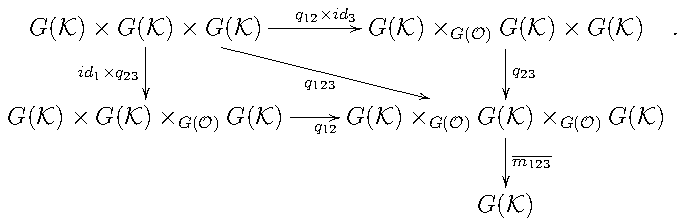
\includegraphics[width=0.5556\paperwidth]{images/L22-p189-associativity.pdf}\end{equation}\end{figure}
$G(\mathcal K)^3$上的$p_G^*\mathcal A_1\boxtimes p_G^*\mathcal A_2\boxtimes p_G^*\mathcal A_3$唯一地下降到
\[G(\mathcal K)\times^{G(\mathcal O)}G(\mathcal K)\times^{G(\mathcal O)}G(\mathcal K),\]
记下降层为$\mathcal D_3$。由\eqref{L22eq15}的交换图，
\[p_G^*((\mathcal A_1*\mathcal A_2)*\mathcal A_3)\cong p_G^*(\mathcal A_1*(\mathcal A_2*\mathcal A_3))\cong Rm_{123*}\mathcal D_3.\]
因此得到以下命题。
\originalnumber{10}
\begin{proposition}\label{L22S1O10}阿贝尔范畴$P_{G(\mathcal O)}(\operatorname{Gr},k)$上由\eqref{L22eq12}定义的卷积积具有自然的结合约束\znote{幺半范畴是带有张量积 $\otimes$ 与单位对象 $\mathbf 1$ 的范畴，并要求结合约束 $\alpha:(X\otimes Y)\otimes Z\cong X\otimes(Y\otimes Z)$ 满足五边形公理、单位约束满足三角形公理；若再给出交换约束 $X\otimes Y\cong Y\otimes X$，便得到对称幺半范畴。本讲在 $P_{G(\mathcal O)}(\operatorname{Gr},k)$ 上验证结合约束（命题 1.10）与交换同构（定理 1.11），这正是把它组织成对称幺半范畴、进而谈论张量等价的前提；卷积的单位对象由 $\operatorname{Gr}_0$ 处的常层给出。[来源：nLab \textquotedbl monoidal category\textquotedbl，\url{https://ncatlab.org/nlab/show/monoidal+category}（Last revised 2025-08-14；2026-11-14 访问）。]}。\end{proposition}
还有以下定理，其证明见\bref{L22MV}{MV}第5节。
\originalnumber{11}
\begin{theorem}\label{L22S1O11}对任意$\mathcal A_1,\mathcal A_2\in P_{G(\mathcal O)}(\operatorname{Gr},k)$，存在自然的交换同构$\mathcal A_1*\mathcal A_2\cong\mathcal A_2*\mathcal A_1$。\end{theorem}
\needspace{5\baselineskip}\section{第22讲参考文献}\label{L22S2}
\begin{references}
\refitem{L22MV}{MV} I. Mirkovi\'c and K. Vilonen, \textit{Geometric Langlands duality and representations of algebraic groups over commutative rings}, Annals of Mathematics, 166 (2007), 95--143.
\end{references}
\sourcepage{190}
\needspace{4\baselineskip}\textbf{关于半小映射。}
\begin{references}
\refitem{L22dCM}{dCM} Mark Andrea A. de Cataldo and Luca Migliorini, \textit{The decomposition theorem, perverse sheaves and the topology of algebraic maps}, \S4.2, available at \url{https://deopurkar.github.io/mhm/dcm.pdf}.
\end{references}
